\documentclass{beamer}
%
% may be included in the beamer package, but just to be sure:
%
\usepackage{graphicx}
% hide subsections+: 1, hide subsubsections+: 2
\addtocontents{toc}{\protect\setcounter{tocdepth}{2}}
% show bookmarks in pdf
\usepackage{hyperref}
% every section (until it has reached the depth of 10 (yeah I overexaggerate with this depth)) will be shown
% in the pdf as a bookmark
%\hypersetup{bookmarksdepth=10}
%
\setbeamertemplate{section in toc}[sections numbered]
\setbeamertemplate{footline}[frame number]
\setbeamertemplate{caption}[numbered]
% dolphin = blue
\usetheme{Madrid}
\usecolortheme{dolphin}
%
\setcounter{secnumdepth}{5}

\makeatletter
\setbeamertemplate{footline}
{
  \leavevmode%
  \hbox{%
  \begin{beamercolorbox}[wd=.4\paperwidth,ht=2.25ex,dp=1ex,center]{author in head/foot}%
    \usebeamerfont{author in head/foot}\insertshortauthor%~~\beamer@ifempty{\insertshortinstitute}{}{(\insertshortinstitute)}
  \end{beamercolorbox}%
  \begin{beamercolorbox}[wd=.266666\paperwidth,ht=2.25ex,dp=1ex,center]{title in head/foot}%
    \usebeamerfont{title in head/foot}\insertshorttitle
  \end{beamercolorbox}%
  \begin{beamercolorbox}[wd=.333333\paperwidth,ht=2.25ex,dp=1ex,right]{date in head/foot}%
    \usebeamerfont{date in head/foot}\insertshortdate{}\hspace*{2em}
    \insertframenumber{} / \inserttotalframenumber\hspace*{2ex} 
  \end{beamercolorbox}}%
  \vskip0pt%
}
\makeatother

\subtitle{Einf\"{u}hrung Simulation}
	\institute{University of Salzburg, Departement of Computer Sciences\\[0.5cm]
		
\includegraphics[scale=0.2]{img/UniLogo.jpeg}		
	}
	\author{Auinger Tobias, M\"{u}ller Christian, Potzkov Georgi}
	\date{\today}
	
%
% + titlepage
%
\begin{document}
\pdfbookmark[1]{Notaufnahme}{title}
\title{Notaufnahme}
\maketitle

	

%
% table of contents
%
\begin{frame}
	\frametitle{Table of contents}
	\pdfbookmark[2]{Table of Contents}{toc}\tableofcontents
\end{frame}

%
\section{Aufgabe}
%
%
\begin{frame}
	\frametitle{Aufgabe:}
	\begin{itemize}
		\item Notaufnahme simulieren
		\item 20 Tage Simulationszeit (+2 Tage Initialisierungsphase)
		\item 2 \"{A}rzte
		\item Drei Patientenpriorit\"{a}ten
	\end{itemize}

\end{frame}

%
\section{Implementierung}
%
%
\begin{frame}
	\frametitle{NewPatientEvent Modell}
	
\includegraphics[scale=1]{img/newPatientEventModell.jpg}
\end{frame}

\begin{frame}
	\frametitle{NewPatientEvent}
	\begin{itemize}
		\item Neuer Patient wird erstellt
		\item 20\% sind Priorit\"{a}t 3
		\item Rest sind Priorit\"{a}t 1
	\end{itemize}		
\end{frame}

\begin{frame}
	\frametitle{PatientArrivalEvent Modell}
	
\includegraphics[scale=1]{img/patientArrivalEventModell.jpg}
\end{frame}

\begin{frame}
	\frametitle{PatientArrivalEvent}
	\begin{itemize}
		\item FreeDoctorQueue leer? 
		\begin{itemize}
			\item ja $\implies$ Sofortbehandlung
			\item nein $\implies$ Queue der jeweiligen Priorit\"{a}t
		\end{itemize}
	\end{itemize}
\end{frame}

\begin{frame}
	\frametitle{TreatmentTermination Modell}
	
\includegraphics[scale=1]{img/treatmentTermination.jpg}
\end{frame}

\begin{frame}
	\frametitle{TreatmentTermination}
	\begin{itemize}
		\item Patient wird behandelt
		\item Behandelnde Arzt $\implies$ BusyDoctorQueue
		\item Berechnen der Behandlungszeit
	\end{itemize}
\end{frame}

\begin{frame}
	\frametitle{Busy/Free Doctor}
	
\includegraphics[scale=1]{img/busyFreeDoctor.jpg}
\end{frame}

%
\section{Erweiterungen}
%
%
\begin{frame}
	\frametitle{Erweiterungen}
	\begin{itemize}
		\item Tod der Patienten
		\item akute Notf\"{a}lle Verdr\"{a}ngen 1 Priorit\"{a}t
	\end{itemize}
\end{frame}

\begin{frame}
	% grafik mit erweiterungen
\end{frame}

\begin{frame}
	% grafik mit erweiterungen
\end{frame}

\begin{frame}
	% grafik mit erweiterungen
\end{frame}



%
%
%
\begin{frame}
	\frametitle{Ergebnisse}
	\begin{minipage}{.5\textwidth}
		\begin{flushleft}		
			\begin{itemize}
				\item[] Zu beachten:
				\item Initial phase
				\item Max. und avg. Wartezeit
				\item \# Patienten die max. 5 Min warten
				\item 90\% Quantile
			\end{itemize}
		\end{flushleft}
	\end{minipage}
	\begin{minipage}{.4\textwidth}
		\begin{flushright}
			\begin{itemize}
				\item[] Zus\"{a}tzlich:
				\item Tode
				\item Bevorzugung der akuten Notf\"{a}lle
			\end{itemize}
		\end{flushright}
	\end{minipage}
\end{frame}

\begin{frame}
	\frametitle{Initial Phase}
\end{frame}

\begin{frame}
	\frametitle{Max. und avg. Wartezeit}
\end{frame}

\begin{frame}
	\frametitle{\# Patienten die max. 5 Min. warten}
	\begin{center}
		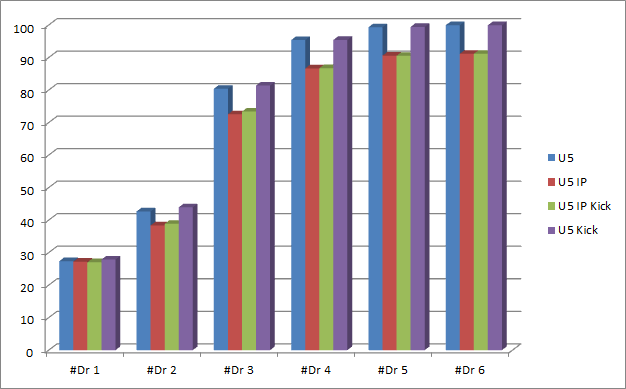
\includegraphics[scale=0.6]{img/U5.png}
	\end{center}
\end{frame}

%\begin{frame}
%	\frametitle{\# Patienten die max. 5 Min. warten}
%	\begin{center}
%		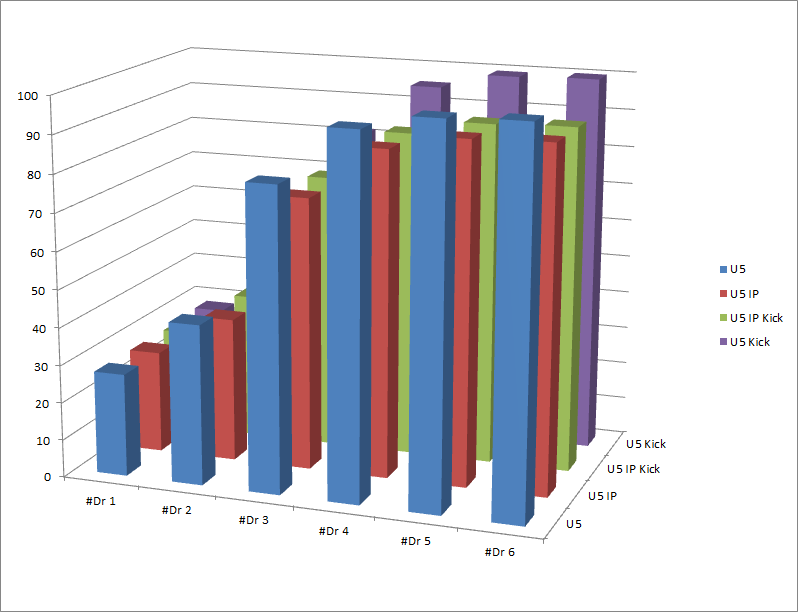
\includegraphics[scale=0.46]{img/U53D.png}
%	\end{center}
%\end{frame}

%\begin{frame}
%	\frametitle{\# Patienten die max. 5 Min. warten}
%	\begin{center}
%		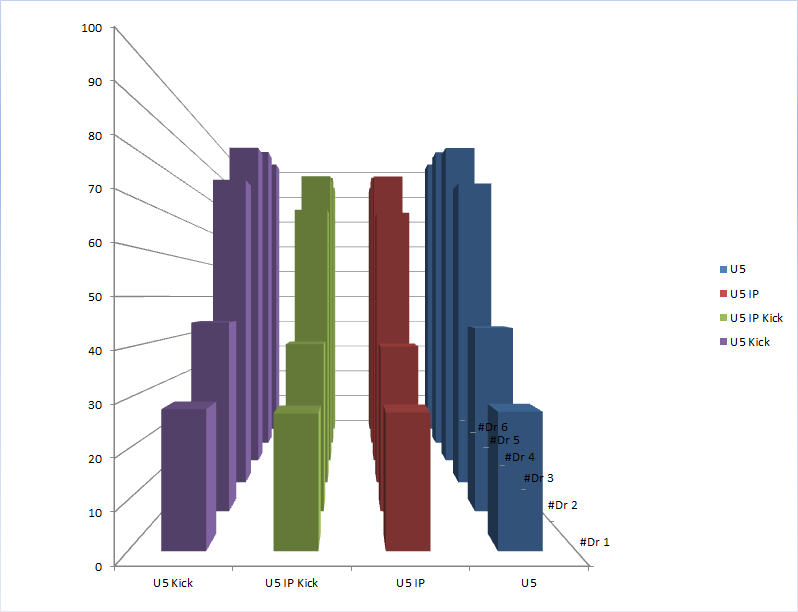
\includegraphics[scale=0.46]{img/U53D2.png}
%	\end{center}
%\end{frame}

\begin{frame}
	\frametitle{90\% Quantile}
\end{frame}

\begin{frame}
	\frametitle{Tode}
	\begin{center}
		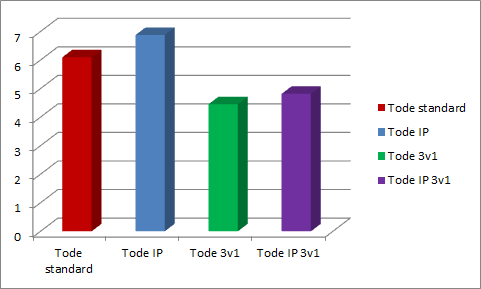
\includegraphics[scale=0.77]{img/Deaths.png}
	\end{center}
\end{frame}

\begin{frame}
	\frametitle{Tode - Nr. Dr}
	\begin{center}
		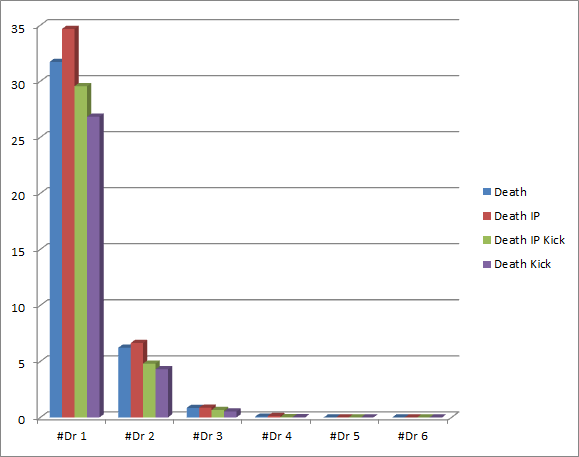
\includegraphics[scale=0.65]{img/DeathsNrDr.png}
	\end{center}
\end{frame}

%\begin{frame}
%	\frametitle{Tode - Nr. Dr}
%	\begin{center}
%		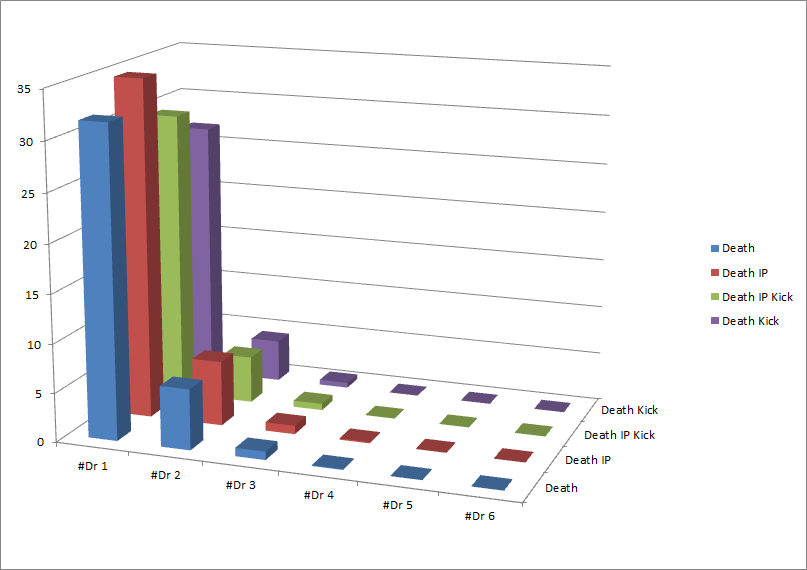
\includegraphics[scale=0.5]{img/DeathsNrDr3D.png}
%	\end{center}
%\end{frame}



\end{document}
